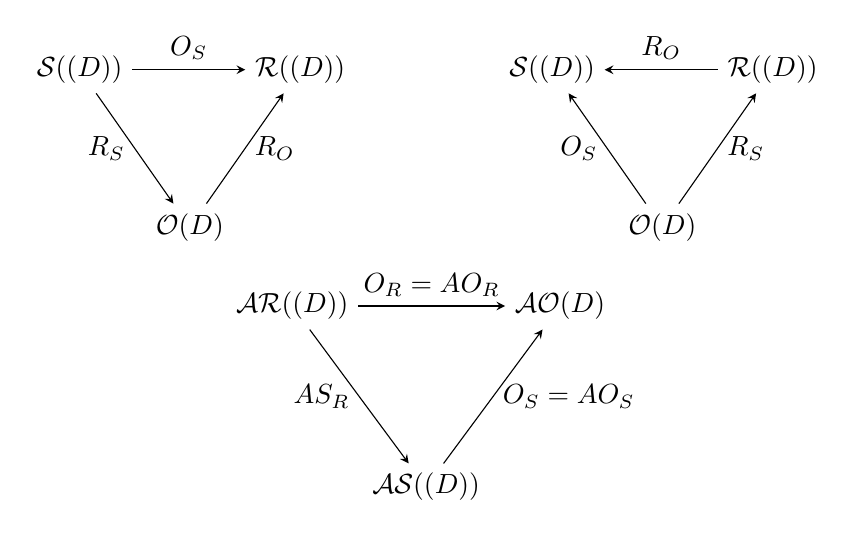
\begin{tikzpicture}

	\node(S1) at (-5.15,0) {$\mathcal{S}(\PP(D))$};
	\node(R1) at (-2.35,0) {$\mathcal{R}(\tc(D))$};
	\node(O1) at (-3.75,-2) {$\mathcal{O}(D)$};
	
	\draw[] (S1) edge [-stealth] node [left]{$R_S$}  (O1);
	
	\draw[] (S1) edge [-stealth] node [above]{$O_S$}  (R1);
	
	\draw[] (O1) edge [-stealth] node [right]{$R_O$}  (R1);
	
	\node at (-3.8,-0.75) {\textbf{\huge{$\circlearrowleft$}}};
	
	\node(R2) at (0.85,0) {$\mathcal{S}(\PP(D))$};
	\node(O2) at (3.65,0) {$\mathcal{R}(\tc(D))$};
	\node(S2) at (2.25,-2) {$\mathcal{O}(D)$};
	
	\draw[] (S2) edge [-stealth] node [right]{$R_S$}  (O2);
	
	\draw[] (S2) edge [-stealth] node [left]{$O_S$}  (R2);
	
	\draw[] (O2) edge [-stealth] node [above]{$R_O$}  (R2);
	
	\node at (2.25,-0.75) {\textbf{\huge{$\circlearrowleft$}}};
	
	\node(S3) at (-2.45,-3) {$\mathcal{AR}(\tc(D))$};
	\node(R3) at (0.95,-3) {$\mathcal{AO}(D)$};
	\node(O3) at (-0.75,-5.3) {$\mathcal{AS}(\PP(D))$};
	
	\draw[] (S3) edge [-stealth] node [left]{$AS_R$}  (O3);
	
	\draw[] (S3) edge [-stealth] node [above]{$O_R=AO_R$}  (R3);
	
	\draw[] (O3) edge [-stealth] node [right]{$O_S=AO_S$}  (R3);
	
	\node at (-0.75,-3.85) {\textbf{\huge{$\circlearrowleft$}}};

\end{tikzpicture}